\chapter{Neuron Segmentation with Tubularity Flow Field} % Main chapter title

\label{TuFF_chapter} % For referencing the chapter elsewhere, use \ref{Chapter2} 

\lhead{Chapter 6. \emph{Tubularity Flow Field}} % This is for the header on each page 

In Chapter \ref{T2T2_chapter} and Chapter \ref{L2S_Ch}, we have discussed two segmentation algorithms. The first method, Tree2Tree-2 is a graph based tracer, which performs neuron tracing by identifying the correct connections between the neurite fragments after an initial segmentation. We remarked in Chapter \ref{T2T2_chapter}, that Tree2Tree-2 encounters difficulties when the neurons exhibit complicated morphology, and it predicts false connections. This motivated us to use geometric active contours, so that the connectivity handling could be performed implicitly. This led to the region based segmentation algorithm L2S, which is primarily designed for 2D applications where the region intensities are inhomogeneous. 

While L2S overcomes the false connectivity problem of Tree2Tree-2, it is essentially a generalized segmentation technique, and we hypothesize that adopting domain specific knowledge in the framework would make neuron segmentation more robust. This motivates our proposed solution, where level sets are used for segmentation, but the energy functional is designed specifically for segmenting tubular structures, both in 2D and 3D.

\section{Introduction}
\begin{figure}[t]
\centering
\includegraphics[width=0.7\linewidth]{./images/TuFF/discontinuities}
\caption[Gaps in neuron structures]{Maximum intensity projection of a neuron imaged by a confocal microscope. The image suffers from contrast non-uniformity, including gaps that lead to breaks in the segmented neurite structure. The effect is most pronounced in the region bounded by yellow dashed box, magnified here for improved viewing.}
\label{fig:discontinuities}
\end{figure}
As earlier, we restrict ourselves to reconstructing single neurons from  confocal microscopy. A robust neuron segmentation scheme needs to address two primary issues. 
\begin{itemize}
\item First, the technique should  be suited to identify neuron structures from the noisy confocal images. This requires a specialized procedure for clutterand noise removal, while preserving the filamentous structures of the neurites. 
\item Second, it should be adept at handling the local structure discontinuities (see Fig. \ref{fig:discontinuities}) resulting from imaging artifacts and pre processing errors. While Tree2Tree-2 used explicit schemes for joining such broken branches, we leverage the capabilities of geometric active contours to do the same.
\end{itemize}
We propose a solution to this segmentation problem using a variational framework driven by geometric active contours. The level set evolution is guided by minimizing an application specific energy functional. A tubularity flow field (TuFF) is computed by utilizing the local tubularity of the neurites which guides the segmentation procedure by encouraging curve evolution along the length (axis) and the thickness of the tubular neurites. A specialized local attraction force is also designed to accommodate the intensity variations in the images of neurite structures, thus presenting an unified framework to naturally link the fragmented structures. Our method does not rely on an initial set of seed-points for segmentation; it is automatic. Moreover, it does not require non-trivial post-segmentation analysis to link the disjoint segments. This is performed naturally by using the local attraction force in a level set paradigm. This enables us to connect disunited structures, even if the underlying signal intensity is significantly low. The problem  formulation and the design process of the attraction force are discussed in the following sections. 

\section{Tubularity Flow Field for neuron segmentation}
Let $f:\Omega \rightarrow \mathbb{R}$ be an image defined on the continuous domain $\Omega \subset \mathbb{R}^d$, where $d$ is the dimension of the image. We propose a solution in a variational paradigm, where implicit motion of the zero level set of the embedding function $\phi$ is obtained by (locally) minimizing an energy functional $\mathcal{E}(\phi)$. 
\begin{figure}[t]
\centering
\subfigure[]{
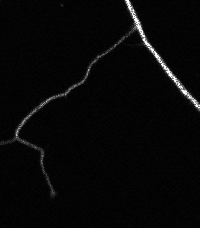
\includegraphics[width=.21\linewidth]{./images/TuFF/n12_speckle}
}
\subfigure[]{
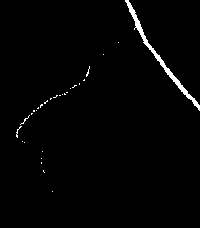
\includegraphics[width=.21\linewidth]{./images/TuFF/n12_Otsu_2}
} 
\subfigure[]{
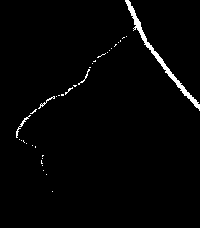
\includegraphics[width=.21\linewidth]{./images/TuFF/n12_ChanVese}
}
\subfigure[]{
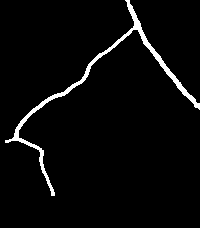
\includegraphics[width=.21\linewidth]{./images/TuFF/MFVF_2}
}

\caption[Global segmentation of neurites]{(a) A 2-D neuron subimage. (b) and (c) show segmentation results using Otsu's method and the Chan-Vese variational technique respectively. Fragmented segmentation output is observed in (b) and (c) due to the non-local behavior of the algorithms. (d) Segmentation using TuFF (the proposed method).}
\label{fig:CV_compare}
\end{figure}
For this problem of neuron segmentation, we need to design the energy functional such that it would encourage curve propagation in the filamentous regions of the image, while avoiding the non tubular structures. Also, the segmentation should allow sufficient local processing to avert fragmented segments in the solution, which may appear as a consequence of using global threshold selection schemes like that of Otsu \cite{otsu} or methods assuming piecewise constant intensity models of \cite{chan_vese} (see Fig.~\ref{fig:CV_compare}).  We avoid this problem  by introducing a local shape prior by way of a specially designed tubularity flow vector field and a local  attraction force  to link nearby neuronal fragments.

\subsection{Tubularity Flow Field (TuFF)}
In Chapter \ref{T2T2_chapter}, we defined the concept of tubularity flow field (TuFF). This vector field consists of the set of orthonormal vectors $\{\textbf{e}_i(\textbf{x})\}$. The vectors are ordered according to increasing magnitude of curvatures, which are given by the scalars $\{|\lambda_i|\}$. We showed in Chapter \ref{T2T2_chapter}, that one popular procedure of obtaining these vector fields is via eigen analysis of the  hessian matrix of the Gaussian  filtered image. Frangi\cite{frangi_vesselness} suggested a multiscale procedure to distinguish vascular structures from background by using a multiscale vesselness function $N(\textbf{x})$. One such choice of a vesselness function is given in (\ref{eq:vesselness_scale}). 

The vesselness function $N(\textbf{x})$ helps distinguishing filamentous structure from noise and clutter, where its value is close to zero.  Clutter are present in most confocal microscopy images due to photon emission from non neuronal tissues and are often referred to as \emph{structure noise}. These structure noise may be bright disc shaped non-neuronal segments in 3D images or blob shaped structures. In the following subsections, we show how TuFF can be incorporated in a level set framework to perform neuron segmentation.

\subsection{Variational formulation with TuFF}
Our method performs segmentation via minimization of the energy functional $\mathcal{E}(\phi)$. This energy functional can be mathematically written as:
\bea
	\mathcal{E}(\phi)&=&\mathcal{E}_{reg}(\phi)+\mathcal{E}_{evolve}(\phi)+\mathcal{E}_{attr}(\phi)
	\label{eq:total_energy} \\
	\mathcal{E}_{reg}(\phi)&=&\nu_1\int_{\Omega}|\nabla H(\phi)|d\textbf{x} 
		\label{eq:smooth_energy}  \\ 
		\mathcal{E}_{evolve}(\phi)&=&-\int_{\Omega}\sum_{i=1}^{d}\alpha_i(\textbf{x})\langle\textbf{e}_i(\textbf{x}),\textbf{n}(\textbf{x})\rangle^2 H(\phi)d\textbf{x}
			\label{eq:evolve_energy}
\eea
Here $\mathcal{E}_{reg}$ and $\mathcal{E}_{evolve}$ are the energy functionals corresponding to the smoothness of the curve and the curve evolution respectively. The functional $\mathcal{E}_{attr}$ contributes towards creating a local attraction energy. This attraction energy is to be designed in a manner such that minimizing it would result in a force field to join the local, disjoint neuron fragments. For our application, we do not define the attraction energy explicitly; instead, we compute the attraction force resultant from the energy. This is discussed in Sec. 6.3.

The vector $\textbf{n}(\textbf{x})=-\dfrac{\nabla\phi(\textbf{x})}{|\nabla\phi(\textbf{x})|}$ denotes the outward unit normal  vector to the level sets of $\phi$. $\langle \cdot,\cdot \rangle$ is the Euclidean inner product operator. The positive scalar $\nu_1$ in (\ref{eq:smooth_energy}) contributes to the smoothness of the zero level curve. The weighing parameter $\alpha_i$ determines the contribution of the orthogonal and axial components of the TuFF in curve evolution. Choice of $\alpha_i$ is an important aspect which would be discussed shortly. 

In practice, the ideal Dirac delta function $\delta(\phi)$ and the Heaviside function $H(\phi)$ are replaced by their regularized counterparts $\dirac(\phi)$ and $\heav(\phi)$ respectively.

\subsection{TuFF gradient flow equation}
The essence of our technique lies in the design of curve evolution energy $\mathcal{E}_{evolve}$ in (\ref{eq:evolve_energy}). In absence of the attraction force energy, the level curve evolution (which results from minimizing the energy term (\ref{eq:evolve_energy})) depends on the contribution of the axial and orthogonal components of the tubularity flow field. The design of the functional (\ref{eq:evolve_energy}) is such that the axial vector field component $\textbf{e}_1$ is responsible for propagating the curve to fill out the vessel thickness. Or in other words, the axial field promotes curve evolution in a direction perpendicular to itself. Identically, the orthogonal components $\textbf{e}_2,\textbf{e}_3$ encourage curve propagation in a direction perpendicular to themselves, i.e. along the axis of the neuron filaments. Let us discuss the effect of tubularity flow field on contour propagation in the following subsection. For simplicity, only a 2D case is discussed, but the extension to 3D follows similar arguments.

\subsubsection{Effect of the axial component of TuFF}
\begin{figure}[t]
\renewcommand{\tabcolsep}{0.05cm}
\begin{tabular}{cc}
	\includegraphics[width=.45\linewidth]{./images/TuFF/tangential_graphic}
	&\includegraphics[width=.45\linewidth]{./images/TuFF/normal_graphic}
	\\
	\scriptsize (a) & \scriptsize (b) 
\end{tabular}
\caption[Graphic illustration of TuFF]{ Illustration of curve evolution due to (a) axial component $\textbf{e}_1$ and orthogonal component (b) $\textbf{e}_2$. Note how the contour should change to align the surface normals (shown in red arrow) with the vector fields (shown in green and purple arrows respectively) to minimize the evolution energy. The initial curve is marked as 1. The evolution forces create the new curves 2. Note how the curves assume elliptical shape to align the level set normals with the vector fields. The normal vectors are maximally aligned in the region enclosed by the rectangles.}
\label{fig:evolve_graphic}
\end{figure}
Maximizing the total squared inner product 
$\displaystyle \int_{\Omega}\alpha_1(\textbf{x})\langle \textbf{e}_1(\textbf{x}),\textbf{n}(\textbf{x})\rangle^2\heav(\phi)$ 
(or minimizing its negative) with respect to the embedding function $\phi$ results in maximally aligning the  outward normal vectors $\textbf{n}(\textbf{x})$ of the zero level sets of $\phi$ and its inner isocontours  with the axial flow field $\textbf{e}_1(\textbf{x})$. This requires the level sets of $\phi$ to be re-aligned such that the normal vectors $\textbf{n}(\textbf{x})$ aligns itself with the axial field $\textbf{e}_1(\textbf{x})$. This results in curve evolution in a direction orthogonal to the vessel axis, causing elongation of the level curves along the vessel width. 

\subsubsection{Effect of the orthogonal component of TuFF}
Using a similar argument, maximizing the second term corresponding to the orthogonal component in (\ref{eq:evolve_energy}) performs alignment of the outward normal vectors with the  vector field $\textbf{e}_2(\textbf{x})$, creating  an elongation force which allows the level curves to propagate along the vessel axis. For an intuitive understanding of the above mentioned phenomenon, Fig.~\ref{fig:evolve_graphic}(a) and (b) is provided to graphically demonstrate how the curve evolution is affected by the axial and the normal components of TuFF. 

\subsubsection{Effect of the vector field weights}
Ideally, the parameters $\alpha_i(\textbf{x}),i=1,\ldots,d,$ should be chosen such that curve propagation is discouraged outside the tubular neurite segments, so as to avoid leakage into the background. i.e. for a voxel $\textbf{y}$ with low vesselness score,  we require $\alpha_i(\textbf{y})\approx 0$, for $i=1,\ldots,d$. Moreover, since the neurites are elongated structures, it is desired that the contour evolution be more pronounced near the filament centerline than at the edges. This can be stated as 
\bea \label{eq:alpha_ratio}
\frac{\alpha_j(\textbf{x})}{\alpha_1(\textbf{x})} \geq 1 \;\; (j=2,\ldots,d)  \;\;\; \text{and}\;\; \alpha_1(\textbf{x}),\ldots,\alpha_d(\textbf{x})>0
\eea
Respecting the above constraints, we propose the following functions for choosing the parameters.
\begin{gather}
\alpha_1(\textbf{x})=N(\textbf{x})\label{eq:alpha1_choice}\\
\alpha_j(\textbf{x})=N(\textbf{x})\left(a_0+\exp\left(-\frac{|\nabla_{\sigma}f(\textbf{x})|}{a_1}\right)^2\right)
\label{eq:alpha2_choice}
\end{gather}
$\forall \textbf{x}\in\Omega$ and  $j=2,\ldots,d$. $N(\textbf{x})$ is the  vesselness score which is obtained from (\ref{eq:vesselness_scale}). 

\subsubsection{Isotropic TuFF equation}
Let us discuss the isotropic case, when $a_0=1$ and $a_1\to \infty$. 
Since the unit normal vector $\textbf{n}(\textbf{x})$  lies in the vector space spanned by $\{\textbf{e}_i(\textbf{x})\}$, it can  be written as $\textbf{n}(\textbf{x})=\displaystyle \sum_{i=1}^{d}m_i\textbf{e}_i(\textbf{x})$. This reduces (\ref{eq:evolve_energy}) to 
\bea
\mathcal{E}_{evolve}(\phi)=-\int_{\Omega}N(\textbf{x})\sum_{i}\langle\textbf{e}_i(\textbf{x}),\sum_{j}m_j\textbf{e}_j(\textbf{x}))\rangle^2 H_\epsilon(\phi)d\textbf{x}
\eea
Since the eigenvectors are orthonormal, $\langle\textbf{e}_i,\textbf{e}_j\rangle=1$ if $\textbf{e}_i,\textbf{e}_j\neq \textbf{0}$ and $i=j$, and 0 otherwise. Also, since $|\textbf{n}(\textbf{x})|=1$, we have $\sum_{i} m_i^2=1$. Using this relation, we obtain $\sum_{i}\langle\textbf{e}_i(\textbf{x}),\sum_{j}m_j\textbf{e}_j(x))\rangle^2=1$. This reduces the evolution equation to
\bea
\mathcal{E}_{evolve}(\phi)=-\int_{\Omega}N(\textbf{x})H_\epsilon(\phi)d\textbf{x}
\label{eq:isotropic_evolve}
\eea
The energy functional in (\ref{eq:isotropic_evolve}) when minimized performs segmentation via vesselness weighted isotropic region growing along the neuron segments. Leakage of the contour outside vessel boundaries is prohibited by the vessel indicator function $N(\textbf{x})$ which provides evidence of tubularity by assuming higher value for the tubular objects than non tubular background.


With the discussion of the isotropic case, it is now easier to visualize the effect of the weights on curve evolution. From our previous discussion, we recall that  $\alpha_1$ and $\{\alpha_j, j\neq 1\}$ influence curve propagation along the vessel width and axial direction respectively.  $|\nabla_{\sigma}f(\textbf{x})|$ denotes the gradient magnitude of the image $f(\textbf{x})$, which is filtered by a Gaussian kernel with variance $\sigma^2$. Since this term is high at the vessel boundaries and end points, the negative exponential term in (\ref{eq:alpha2_choice}) ensures higher response at regions near the vessel centerline. The tuning parameters $a_0 \ge 1$ and  $a_1$ determine the relative influence of the axial curve motion to the motion along the vessel width.  In other words, in an anisotropic setting, (\ref{eq:alpha2_choice}) suggests that  the level curves evolve with higher curvature near the vessel medial axis than at  the  edges, which percolates to the isotropic case when $a_0=1$ and $a_1\to \infty$. 

Since the neurite filaments are predominantly thin, elongated structures, we observe that  the isotropic case yields sufficiently appropriate segmentation results when the initialized zero level set encompasses the filament width. Nevertheless, the proposed framework in (\ref{eq:total_energy}) is general, and is applicable to segmentation problems where vessel thickness is significant and the initialized zero level contour does not fill out the vessel width completely. This is in contrast to the approach in \cite{shang2011vascular}, where segmentation of thicker vessels needs separate treatment. 

\subsection{Minimization of the TuFF functional}
The energy functional in (\ref{eq:total_energy}) can be minimized using variational calculus techniques \cite{calc_of_var}. Taking the G{\^a}teaux variation of $\mathcal{E}(\phi)$ with respect to $\phi$, we obtain from (\ref{eq:total_energy})
\begin{align}
	\nabla_\phi \mathcal{E} =\nabla_\phi \mathcal{E}_{reg}+\nabla_\phi \mathcal{E}_{evolve}+\nabla_\phi \mathcal{E}_{attr}
\label{eq:gateaux}
\end{align}
$\phi$ can be iteratively updated using gradient descent technique, i.e. setting $\nabla_\phi \mathcal{E}=-\dfrac{\partial\phi}{\partial t}$ with $t$ denoting the pseudo time parameter for the iterative scheme:
\bea\label{eq:total_force_eqn}
\frac{\partial\phi}{\partial t}=\mathcal{F}_{reg}(\textbf{x})+\mathcal{F}_{evolve}(\textbf{x})+\mathcal{F}_{attr}(\textbf{x})
\eea
$\mathcal{F}_{reg}$ and $\mathcal{F}_{evolve}$ are scalar force functions, which resulting from locally minimizing the regularizing energy and the evolution energy functionals. These forces are derived by solving the  Euler-Lagrange equation for level set evolution in the following manner:
\bea
	\mathcal{F}_{reg}(\textbf{x})&=&\nu_1 \, \text{div}\left(\textbf{n} \right)\dirac(\phi) \label{eq:reg_force}\\
	\mathcal{F}_{evolve}(\textbf{x})&=&\dirac\left(\phi\right)\sum_{j=1}^{d}\{\alpha_j(\textbf{x})\beta_j^2\left(\textbf{x} \right)\}- \nn\\
	&& 2\;\rm{div}\left(\sum_{\mathit{j}=1}^{\mathit{d}}\eta_{\mathit{j}} (\textbf{x})\left(\textbf{v}_j(\textbf{x})-\beta_{\mathit{j}} \left(\textbf{x}\right)\textbf{n}(\textbf{x})\right)\right) \nn\\
	\label{eq:evolve_force}
\eea
The coefficients $\beta_j$ and $\eta_j$ are defined as follows:
\bea
	\beta_j(\textbf{x})&=&\langle \textbf{v}_j(\textbf{x}),\textbf{n}\left(\textbf{x}\right)\rangle \\
	\eta_j(\textbf{x})&=&\alpha_j(\textbf{x})\beta_j(\textbf{x})\dfrac{\heav(\phi)}{|\nabla \phi|}
\eea 
The derivation details are shown in Appendix \ref{AppendixTuFF}.

\section{Local attraction force field}
The attraction force $\mathcal{F}_{attr}$ in (\ref{eq:total_force_eqn}) is introduced to accommodate the signal intensity variation (and signal loss) across the neurite branches, as shown in  Fig.~\ref{fig:discontinuities}. Such signal attenuation introduces unwarranted discontinuities in the filamentous objects, resulting in disjoint fragments.
Also, discontinuities may be present at the neurite junctions and noisy regions due to the nonlinear response of the vesselness function in (\ref{eq:vesselness_scale}). In such a scenario, the TuFF based evolution energy term in (\ref{eq:evolve_energy}) is not adequate by itself to perform segmentation. This insufficiency motivates the inclusion of an attraction force component. Designing this attraction force requires analysis of the connected components at each time epoch of level set propagation. At a time $t$ for evolution of the embedding function, the set of connected components $\mathcal{C}(t)$ are obtained as: 
\bea
	\mathcal{C}(t)=H\left(\phixt \right) \\
	\text{where $H(y)=$}\nn
	\begin{cases}
		1 & \text{for $y\geq0$}\\
		0 & \text{$y<0$}
	\end{cases}
\eea
The set of connected components $\mathcal{C}(t)=\{c_1,\ldots,c_p\}$ represents the binary segmentation at time $t$, which consists of $p\geq1$ disjoint connected components. Note that this binarization does not require a sophisticated segmentation, since the binary components are obtained by extracting the interior of the zero level sets of the embedding function. Each disjoint component $c_j$ is a potential candidate or a \emph{parent} which has the capability of attracting the remaining \emph{children} $c_k$, 
$k\ne j$,$\left(j,k= 1,\ldots,p\right)$. This is illustrated in Fig.~\ref{fig:attr_force}(a)-(c), where the component $c_1$ acts as a parent component and $c_2$ and $c_3$ are the children.
\begin{figure}[t]
\centering
\subfigure[]{
		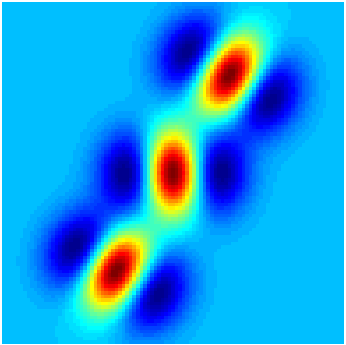
\includegraphics[width=.31\linewidth]{./images/TuFF/attr_force/all}
}\hspace{-0.2cm}
\subfigure[]{
		\includegraphics[width=.31\linewidth]{./images/TuFF/attr_force/CH_master}
}\hspace{-0.2cm}
\subfigure[]{
		\includegraphics[width=.31\linewidth]{./images/TuFF/attr_force/slaves}
}\hspace{-0.2cm}
\\
\centering
\subfigure[]{ %
	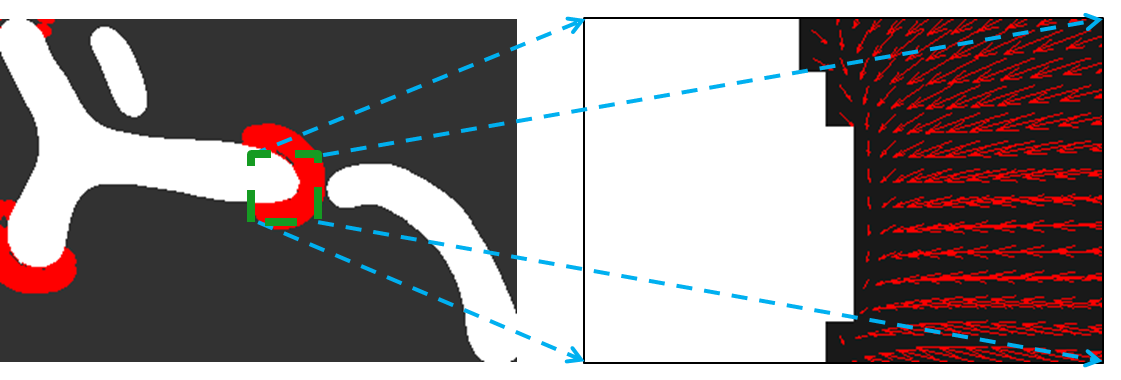
\includegraphics[width=0.7\linewidth]{./images/TuFF/attr_force/force_field}
}
\caption[Graphic illustration of local attraction force field]{(a) Set of disjoint connected components $\{c_1,c_2,c_3\}$ at a particular step of iteration. (b) shows a parent component, the green dotted line marking its convex hull. The remaining children are shown in (c). (d) shows the attraction force obtained via (\ref{eq:Attr_Field}) in red arrows, magnified for visual clarity.}
\label{fig:attr_force}
\vspace{-0.2in}
\end{figure}

\subsection{Candidate points for attraction force field}
The primary responsibility of the attraction force is to enable the propagating contour surface to attach itself to local disjoint fragments. However, not all points on the connected components are candidates for creating the attraction force. This is because in a majority of the prevalent discontinuities, at least one of the two disconnected portions are likely to be joined via boundary points which represent region of high curvature (see Fig.~\ref{fig:disc_types}). 
If we denote the boundary of a component $c_j$ by $\delta c_j$, to enable a parent to attract a child, we need to design an attraction field which is generated by a set of candidate points lying on the parent boundary. 
Therefore, for a parent component $c_j$, a point $\textbf{y}\in \delta c_j$ belongs to the candidate set if $\textbf{y}$ is a point the convex hull \cite{convex_hull_graham} $\mathcal{H}_j$  of $c_j$ (Fig.~\ref{fig:attr_force}(b)). Formally, the candidate point set $\mathcal{M}_j$ for the connected component $c_j$ is defined as
\bea
\mathcal{M}_j=\{\textbf{y}\in \delta c_j:\exists \:\textbf{x}_j \in \mathcal{H}_j \;\; \text{s.t.}\; \|\textbf{y}-\textbf{x}_j\|_2\leq \Delta\}
\eea
$\Delta$ is a positive parameter that includes local boundary coordinates of the neighboring points on the convex hull. 

\subsection{Attraction force field design}
The candidate set of points for a parent component is responsible for generating a force field capable of attracting the candidate children towards itself for potential merging. This needs to be designed such that the attraction field vectors point toward the region of interest, which is the parent candidate point set for this purpose. We show that an efficient solution may be obtained by using vector field convolution (VFC) to create the attraction force field.

VFC \cite{li_VFC} is a technique primarily designed to create smooth external force field for parametric active contours. The specially designed vector field kernel (\ref{eq:VFC}) generates the desired external force when convolved with the object edge map, with the capability of attracting a contour to the region of interest.
\bea
	\textbf{K}(\textbf{p})=&-m(\textbf{p})\frac{\textbf{p}}{\|\textbf{p}\|} \nn\\
%	m(\textbf{p})&=&\|\textbf{p}\|^{-\gamma}
	m(\textbf{p})=&\exp(-||\textbf{p}||^{2}/\gamma^{2})
	\label{eq:VFC}
\eea
$\textbf{p}=\bf 0$ denotes the kernel center. The capture range of the vector field is controlled by the parameter $\gamma$. 

The set of candidate points $\mathcal{M}_j$ for a parent $c_j$ serves as the region of interest to which other components are likely to be attracted. Performing convolution of the candidate set with the kernel in (\ref{eq:VFC})  results in a vector field where the vectors are directed toward the parent, their magnitude attenuating gradually with distance from the candidate set.
If $E_j(\bf x)$ is a binary edge-map which assumes a value of $1$ only at points in $\mathcal{M}_j$, we can obtain the attraction force field  $\Gamma_j$ due to the parent $m_j$ as
\bea
\label{eq:Attr_Field}
\Gamma_j(\textbf{x})=E_j(\textbf{x})\ast \textbf{K}(\textbf{x}), \quad \forall \textbf{x}\in \Omega.
\eea
The nature of the attraction force field can be intuitively understood from Fig.~\ref{fig:attr_force}. Fig.~\ref{fig:attr_force}(a)  shows three connected components and the representative parent $c_1$ enclosed by its convex hull (shown in (b)). Fig.~\ref{fig:attr_force}(c) illustrates the attraction force field due to the parent as the red arrows which are oriented in the direction of the parent component. The capture range, which is specified by $\gamma$, is shown by the red region. 

Adopting this policy for designing the attraction field enjoys a few benefits. First, with a specified capture range, we can impose a locality in the approach, by discouraging distant segments to be connected to the parent. As $\gamma$ increases, effect of the attraction force field gradually diminishes as one moves further from the parent. Moreover, the candidate set is chosen such that only the convex portions of the parent boundary are capable of generating the force field. This ensures not all local structures are potential candidates for linking. For example, in Fig.~\ref{fig:attr_force} the component $c_3$ is not in the capture range of the force field of $c_1$, although it resides in the parent's local neighborhood. To summarize, the attraction force field is designed such that it may attract local connected components which are present in near vicinity of the parent's boundary convexity.  

\subsection{Attraction force}
For a parent-child pair $c_i$ and $c_j$, the parent attracts the child with a force $\mathcal{F}_{attr}^{(i,j)}$ given by
\bea
\mathcal{F}_{attr}^{(i,j)}(\textbf{y})=\mathcal{M}_i\langle \Gamma_i(\textbf{y}),-\textbf{n}(\textbf{y})\rangle \theta_j(\textbf{y})
\label{eq:attr_force_ij}
\eea
The indicator function $\theta_j(\textbf{y})=1$ if $\textbf{y}\in \delta c_j$ and $0$ otherwise. $\mathcal{M}_i$ is the normalized mass of the component $c_i$ which is computed as the ratio of the number of pixels/voxels in $c_i$ to the total pixels/voxels in $\{c_1,\ldots,c_p\}$. The inner product term in (\ref{eq:attr_force_ij}) suggests that higher force of attraction is experienced by a point on a child's boundary if the outward normal at that point is oriented along the attraction field.  


By introducing the factor $\mathcal{M}_i$, we equip heavier connected components with more attractive power.
Assuming that the neurites occupy larger volume than the noisy background voxels, we clean the solution of the level set function by performing an area opening operation which eliminates small components with area less than a pre defined threshold \cite{acton_fast}. This filtering operation avoids undesired objects to participate in the attraction force field computation. Now, for each parent-child pair in the filtered component space, we can compute the total attraction force $\mathcal{F}_{attr}$ in (\ref{eq:total_force_eqn}) as
\bea
\mathcal{F}_{attr}(\textbf{y})=\nu_2\sum_{i=1}^{p}\sum_{j\neq i}^{p}\mathcal{F}_{attr}^{(i,j)}(\textbf{y}),\quad
\forall \textbf{y}\in \Omega.
\label{eq:total_attr_force}
\eea
The positive scalar $\nu_2$ determines the effect of the attraction force on curve evolution. A finite difference scheme is used to solve the PDE in (\ref{eq:total_force_eqn}) with initial value obtained using Otsu's global segmentation \cite{otsu} and Neumann boundary condition. 

\section{Handling of discontinuities}
Typically, one may encounter two major sources of structure discontinuity arising from initial segmentation. Fig.~\ref{fig:disc_types} shows three synthetic, disjoint components at an arbitrary stage of level set evolution. The type A discontinuity occurs when connectivity is absent between the end points or leaves of the centerline of the respective objects. Type A discontinuities dominate our application, and connectivity analysis of type A  may be performed via Tree2Tree \cite{basu_T2T_journal}, by investigating the geometric orientation and Euclidean distance between the end points . 
\begin{figure}[t]
\centering
\includegraphics[width=.6\textwidth]{./images/TuFF/attr_force/discontinuities}
\caption[Type A and Type B discontinuities]{Two types of discontinuities between the disjoint components. The \emph{Type A} discontinuity can be resolved by joining the end points of the center lines of the respective branches. \emph{Type B} is more difficult, where discontinuity occurs between a branch end point and an intermediate point on the centerline of the other branch.}
\label{fig:disc_types}
\end{figure}
However, end-point analysis algorithms like Tree2Tree are unable to process the type B discontinuities, where the link needs to be established between the terminal node of one component with a non-terminal point on the other object. This problem is persistent in Tree2Tree-2 also, since the algorithm eventually uses the explicit connectivity determination step to link the neurite subcompartments.
This is where the proposed level set framework wins over conventional component linking algorithms since level sets are proficient in handling topological changes of the evolving segmentation.


\subsection{Type A discontinuities}
Type A discontinuities are relatively simpler to analyze. If the neuron filament signal intensity is uniform, then the evolution force component of (\ref{eq:total_force_eqn}) sufficiently propagates the level sets until they are finally merged. However, when the signal drop is substantial, the attraction force term in (\ref{eq:total_force_eqn}) assists the parent and the child component to exert attractive forces on one another, thus propagating the curves till they merge. A demonstration is shown in the first row of Fig.~\ref{fig:typeAB_demo}. The initial segmentation using Otsu's method creates type A gaps, which are ultimately merged. We have intentionally eliminated a portion of the neuron's branch to demonstrate that our methodology works even in complete absence of signal. 

\begin{figure}[t]
\centering
\renewcommand{\tabcolsep}{0.02cm}
\begin{tabular}{ccccccc}
	\includegraphics[width=.14\linewidth]{./images/TuFF/TypeB_demo/TypeA/1} &
	\includegraphics[width=.14\linewidth]{./images/TuFF/TypeB_demo/TypeA/2} &
	\includegraphics[width=.14\linewidth]{./images/TuFF/TypeB_demo/TypeA/3} &
	\includegraphics[width=.14\linewidth]{./images/TuFF/TypeB_demo/TypeA/4} &
	\includegraphics[width=.14\linewidth]{./images/TuFF/TypeB_demo/TypeA/5} &
	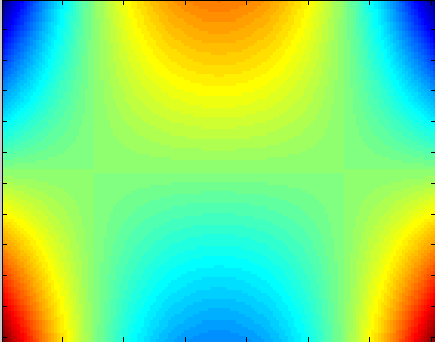
\includegraphics[width=.14\linewidth]{./images/TuFF/TypeB_demo/TypeA/6} &
	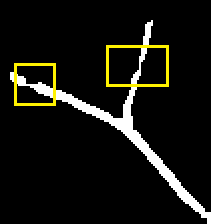
\includegraphics[width=.14\linewidth]{./images/TuFF/TypeB_demo/TypeA/converged} 
	\\
	\includegraphics[width=.14\linewidth]{./images/TuFF/TypeB_demo/TypeB/1} &
	\includegraphics[width=.14\linewidth]{./images/TuFF/TypeB_demo/TypeB/2} &
	\includegraphics[width=.14\linewidth]{./images/TuFF/TypeB_demo/TypeB/2_5} &
	\includegraphics[width=.14\linewidth]{./images/TuFF/TypeB_demo/TypeB/3} &
	\includegraphics[width=.14\linewidth]{./images/TuFF/TypeB_demo/TypeB/4} &
	\includegraphics[width=.14\linewidth]{./images/TuFF/TypeB_demo/TypeB/5} &
	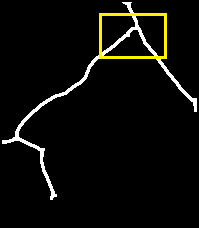
\includegraphics[width=.14\linewidth]{./images/TuFF/TypeB_demo/TypeB/converged} \\
	\scriptsize (a)	& 	\scriptsize (b) & 	\scriptsize (c)	& 	\scriptsize (d) &	\scriptsize (e)	& 	\scriptsize (f) &   \scriptsize (g)
\end{tabular}
\caption[TuFF performance with discontinuities]{(a) and (b) shows the original image and the initial global segmentation respectively for two cases demonstrating handling of Type A (top row) and Type B (bottom row) discontinuities. (c)-(f) shows segmentation at subsequent time intervals. (g) shows the final segmentation, where the structure gaps have been closed (the merged portions are enclosed in rectangles). }
\label{fig:typeAB_demo}
\end{figure}
\subsection{Type B discontinuities}
Type B discontinuity involves two segments, for which connectivity needs to be established between one component's end point (or tip) with the other component's body. In presence of adequate signal intensity, TuFF drives the geometric contours toward the participating structure as per the filament orientation. However, when signal intensity drops, the attraction force takes over. An example is shown in the second row of Fig.~\ref{fig:typeAB_demo}(b), where the initial segmentation creates a type B gap. The situation is different from that of type A, where both the components may attract each other. In case of type B, only one component can assume a parent's role. Note that this is the extreme scenario, where the underlying signal strength is so feeble that it renders the evolution force term useless. However, assuming that the parent's mass is not negligible, this attraction force is strong enough to pull the local child connected component for potential merging. It should be noted that only those regions on the child's boundary whose outward normals are maximally aligned with the exerted force field are attracted toward the parent. 

\section{Curve evolution equation}

Numerical implementation of (\ref{eq:total_force_eqn}) allows iterative computation of the level set function, which can be expressed as
\bea 
\phi^{(k+1)} = \phi^{(k)} + \Delta t\mathcal{L}^{(k)}
\eea
The learning rate $\Delta t$ is fixed to a small value $(\approx 0.1)$ to allow stable computation. $\mathcal{L}^{(k)}$ denotes the discretized version of the right hand side of (\ref{eq:total_force_eqn}). $\phi^{(k)}$ is the level set function at iteration $k$. 
To initialize the active contour, we require the initialized curve to be inside the neurite structure. The initial level set function may be easily obtained via few mouse clicks to select a region inside the neuron structure. However, to avoid this human involvement, we perform a global thresholding of the scale space vesselness image (\ref{eq:vesselness_scale}) using Otsu's technique \cite{otsu}, followed by noisy binary segment removal using the area open filter \cite{acton_fast}. The iterative procedure is halted when no significant change in the length of the zero level curve of $\phi$ is observed. At convergence, the neuron structure is extracted by selecting the largest binary component in the solution. A cubic spline is then fitted to each branch of the obtained centerline to obtain  smooth tracing of neuron centerline. 

\section{Experimental results}
To evaluate the performance of TuFF, we set up experiments for segmenting neurons from both 2D and 3D images. As we have mentioned earlier, 2D analysis often serves as the first step for neuron morphological studies. Plus, certain categories of neurons (such as the ones in the cuticle layer) exhibit a flat geometry, and in such cases the extra dimension does not add significant information about their structure. In this section, qualitative segmentation results (for both 2D and 3D images) will be presented first, with an emphasis on some salient properties of TuFF such as segmentation in presence of severe signal attenuation and robustness against Type B connectivity errors. The quantitative results of neuron tracing will be then furnished, with a suitable similarity metric, calculated against manually obtained results.

\subsection{Dataset for segmentation}
We test the performance of TuFF segmentation algorithm on sets of 2-D and 3-D confocal microscopy images. The 2-D images are primarily used to demonstrate the efficacy of TuFF over component analysis algorithms like Tree2Tree \cite{basu_T2T_journal}. The 3-D image data set consists of confocal microscopy images of the Drosophila larva, which are genetically tagged with green fluorescence protein (GFP). A majority of the neurons have been imaged in Dr. Barry Condron's laboratory at the University of Virginia, department of Biology.   The images are captured using a laser scanning confocal microscope and has a horizontal pixel width of $0.14 \mu m$ and vertical pixel width of $0.18 \mu m$. These images are characterized by intense background clutter from non neuronal objects (such as the food particles, mildly fluorescing tissues etc.) and considerable contrast and intensity variation. This dataset will be referred to as \textit{Condron dataset}.

The second data set for 3-D analysis consists of olfactory (axonal) projection (OP) image stacks of Drosophila larva. These images were used in the Diadem challenge \cite{diadem_dataset} and like the previous dataset, these neurons are also imaged by a confocal microscope. These \textit{OP-dataset} images are less noisy (due to a noise reduction technique which is inbuilt in the imaging software) and the contrast is better than the images in Condron data set. However, the neurons in this data set exhibit acutely complicated structural appearance in addition to occasional intensity heterogeneity along the neurite filaments.

\subsection{Parameter selection}
\begin{figure}[t]
\centering
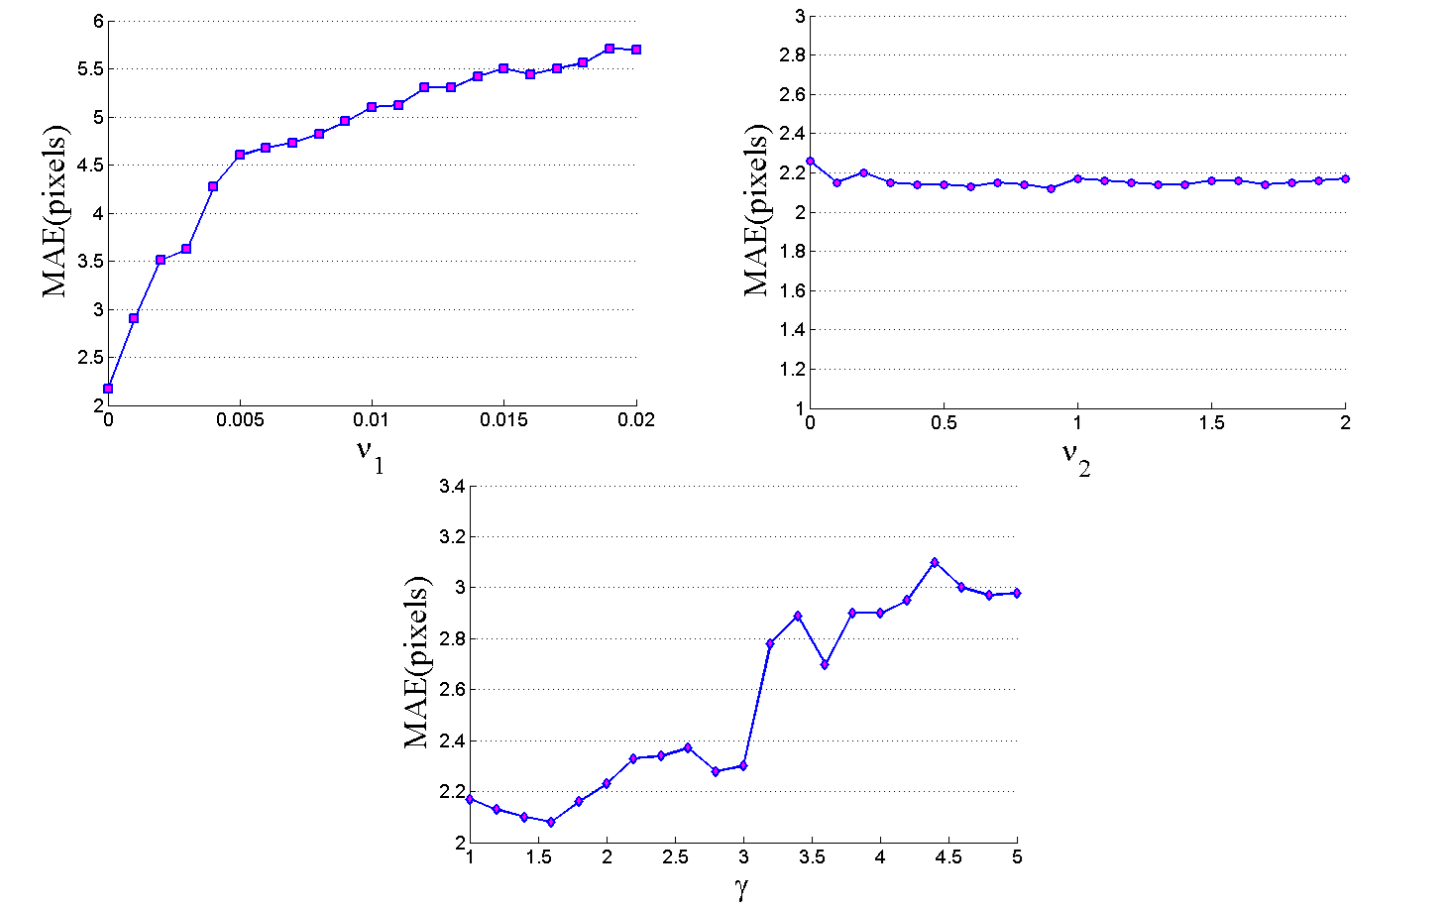
\includegraphics[width=0.8\linewidth]{./images/TuFF/parameter}
\caption[Parameter sensitivity analysis]{Sensitivity analysis of the parameters. The mean absolute error of the traced centerline are plotted in the vertical axis for different values of the tuning parameters.}
\label{fig:param}
\end{figure}

The level set evolution equation (\ref{eq:total_force_eqn}) depends on a few parameters. The evolution force $\mathcal{F}_{evolve}$ requires specifying the positive scalars $a_0$ and $a_1$ in (\ref{eq:alpha2_choice}) which controls the anisotropy of curve evolution. As we have discussed before, since the neurite thickness in our case does not vary considerably, we have adopted the isotropic case, as it requires lesser computation. Therefore, we choose $a_0=1$ and a sufficiently high value for $a_1$. 


The smoothness of the evolved curve is controlled by the parameter $\nu_1$ in (\ref{eq:evolve_force}). Effect of gradually increasing $\nu_1$, keeping other parameters fixed results in an increased mean absolute error in tracing, as shown in Fig.~\ref{fig:param}. For our experiments, $\nu_1$ is fixed at a value in the range $0-0.02$.

The attraction force defined in (\ref{eq:total_attr_force}) depends on the weighing parameter $\nu_2$ and the parameter $\gamma$ controlling the local capture range. As we observe in Fig.~\ref{fig:param} our algorithm is relatively robust to the choice of $\nu_2$. However, we notice that a very low value of $\nu_2$ restricts the attraction force from closing small gaps. For all our experiments, we select $\nu_2=1$.  The term $\gamma$ induces locality in the capture range for the attraction force. While a small value of $\gamma$ can be too restrictive, a relatively high value attracts distant structures to be merged to the attracting component (see Fig.~\ref{fig:param}).  Note that we are interested in connecting the disjoint structures over a local neighborhood. Based on our knowledge about the dataset, we observe that typically $\gamma$ ranges between $0.2-1.5\mu m$ ($\approx$ 1--7 pixels) for our data. Setting these biologically inspired bounds on the range of $\gamma$, we proceed to select the value in the following manner. First, at any stage of segmentation, we compute the median distance $\rho$ between all the segments, and update the value of $\gamma$ as $\gamma^*=\mathcal{\rho}/3$. If the updated value is beyond the pre selected upper or lower bounds, we select the closest boundary value for $\gamma^*$. This is repeated at each iteration to compute the attraction  force.

Experimentally we have observed that the parameters $\Delta$ and $\epsilon$ can be prefixed to a particular value without affecting performance. For all experiments we choose $\Delta=5$ pixels and $\epsilon=1$ as suggested by the authors in \cite{chan_vese}.

\subsection{2D segmentation via TuFF: qualitative results}
Fig.~\ref{fig:Ascoli2D} demonstrates the efficacy of TuFF in segmenting flat neuron cells from the subcuticle layer of Drosophila larva. The maximum intensity projection images of the neurites are shown in Fig.~\ref{fig:Ascoli2D}(a1) and Fig.~\ref{fig:Ascoli2D}(a2), and the respective segmentation results are shown in Fig.~\ref{fig:Ascoli2D}(b2) and (c2). 

This example suggests that using TuFF, segmentation of vascular structures can be performed robustly, without extensive human intervention. The above shown images exhibit low contrast with significant filament discontinuities, and the neuronal processes have significant structural complexity with numerous branches and bifurcations. 

\begin{figure}[t]
\centering
\renewcommand{\tabcolsep}{0.05cm}
\begin{tabular}{cc}
	\includegraphics[width=.49\linewidth]{./images/TuFF/2D_results/left} &
	\includegraphics[width=.49\linewidth]{./images/TuFF/2D_results/left_seg} \\
	\scriptsize (a1) & \scriptsize (b1)
\end{tabular}
\begin{tabular}{c}
	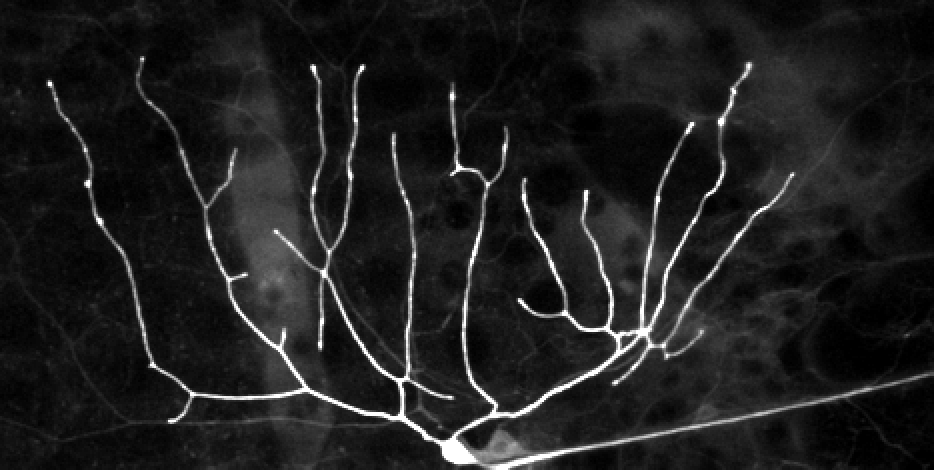
\includegraphics[width=.9\linewidth]{./images/TuFF/2D_results/ascoli_2_mip} \\
	\scriptsize (a2) \\
	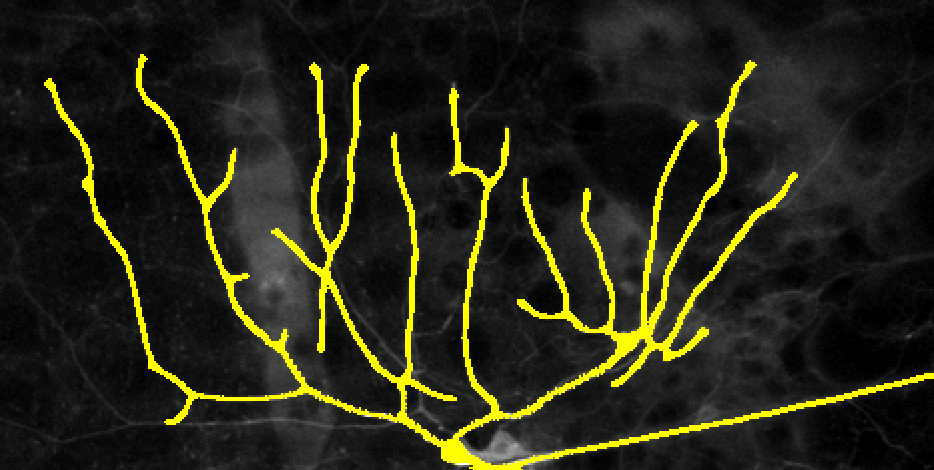
\includegraphics[width=.9\linewidth]{./images/TuFF/2D_results/Ascoli_initial_res_y} \\
	\scriptsize (b2)
\end{tabular}
\caption[TuFF for subcuticle layer neurons]{Segmentation of 2D flat neuron cells using TuFF. The images are courtesy Dr. G. Ascoli's lab, George Mason University, USA.}
\label{fig:Ascoli2D}
\end{figure}
\clearpage

\subsection{Efficacious handling of branch connectivity}
\begin{figure}[h]
\renewcommand{\tabcolsep}{0.05cm}
\begin{tabular}{ccc}
	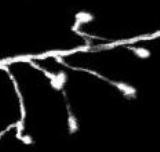
\includegraphics[width=.32\linewidth]{./images/TuFF/TypeB_demo/neuron9_cropped}
	&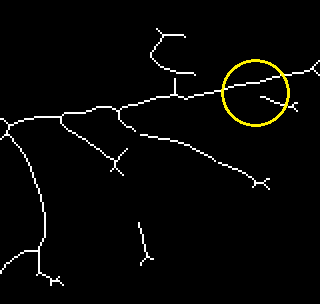
\includegraphics[width=.32\linewidth]{./images/TuFF/TypeB_demo/demo2_skel}
	& 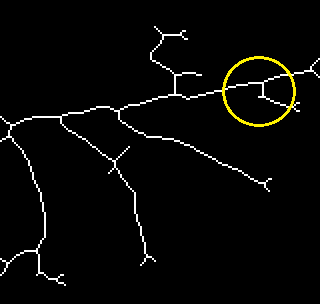
\includegraphics[width=.32\linewidth]{./images/TuFF/TypeB_demo/demo2_postSeg}
	\\
	\scriptsize (a) & \scriptsize (b) & \scriptsize (c)
\end{tabular}
\centering
\begin{tabular}{cc}
	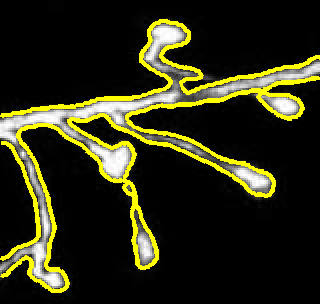
\includegraphics[width=.325\linewidth]{./images/TuFF/TypeB_demo/demo2_segmented}
	&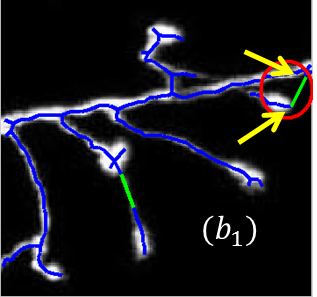
\includegraphics[width=.33\linewidth]{./images/TuFF/2D_results_2/b1} \\
	\scriptsize (d) TuFF & \scriptsize (e) Tree2Tree
\end{tabular}
\caption[TuFF vs Tree2Tree]{(a) 2-D neuron sub-image. (b) Centerline of the initial segmentation using \cite{otsu}. The type B discontinuity is highlighted by the yellow circle. (c) Centerline obtained after segmentation using TuFF. (d) Final segmentation via TuFF. (e) Tracing using Tree2Tree. A typical error in connectivity is indicated by the arrows.}
\label{fig:Tuff_vs_T2T}
\end{figure}
Previously, we have demonstrated the ability of TuFF to handle type A and type B discontinuities. In this section, we demonstrate the advantage of using TuFF over Tree2Tree \cite{basu_T2T_journal} for determining branch connectivity. For this purpose, we show segmentation results on a few 2-D neuron images. The 2-D images are obtained from a maximum intensity projection of the corresponding 3-D stacks.
\begin{figure}[t]
\centering
\renewcommand{\tabcolsep}{0.05cm}
	\begin{tabular}{@{}ccc @{}}
		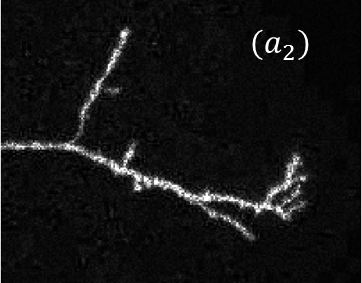
\includegraphics[width=.31\linewidth]{./images/TuFF/2D_results_2/a2} &
		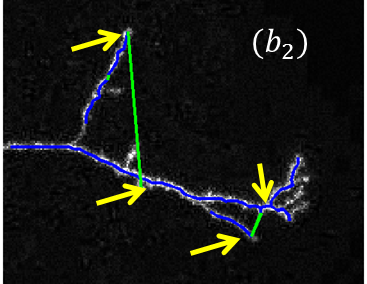
\includegraphics[width=.31\linewidth]{./images/TuFF/2D_results_2/b2} &
		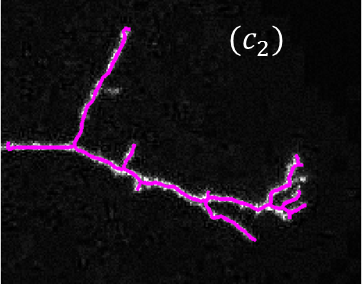
\includegraphics[width=.31\linewidth]{./images/TuFF/2D_results_2/c2} \\
		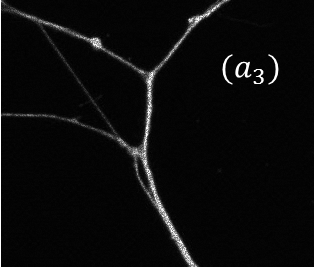
\includegraphics[width=.31\linewidth]{./images/TuFF/2D_results_2/a3} &
		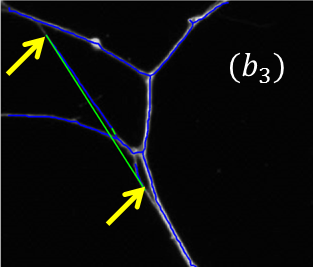
\includegraphics[width=.31\linewidth]{./images/TuFF/2D_results_2/b3} &
		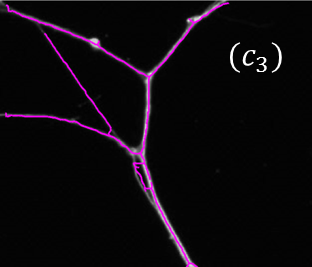
\includegraphics[width=.31\linewidth]{./images/TuFF/2D_results_2/c3} \\
		\scriptsize (a) MIP image & 		\scriptsize (b) Tree2Tree & 		\scriptsize (c) TuFF
	\end{tabular}
\caption[TuFF vs Tree2Tree for Type B error (2D)]{The first column shows sample 2-D neuron images. Tree2Tree \cite{basu_T2T_journal} segmentation results are displayed in the second column. The edges linked by Tree2Tree are shown in green and the traced centerline is overlaid on the original image in blue. Excessive clutter restricts the efficiency of Tree2Tree, yielding improper connections, which are highlighted by the yellow arrows. The last column shows tracing output via TuFF (magenta).}
\label{fig:twoD_comp_i}
\end{figure}

\begin{figure}[h]
\centering
\renewcommand{\tabcolsep}{0.05cm}
	\begin{tabular}{@{}c @{}}
		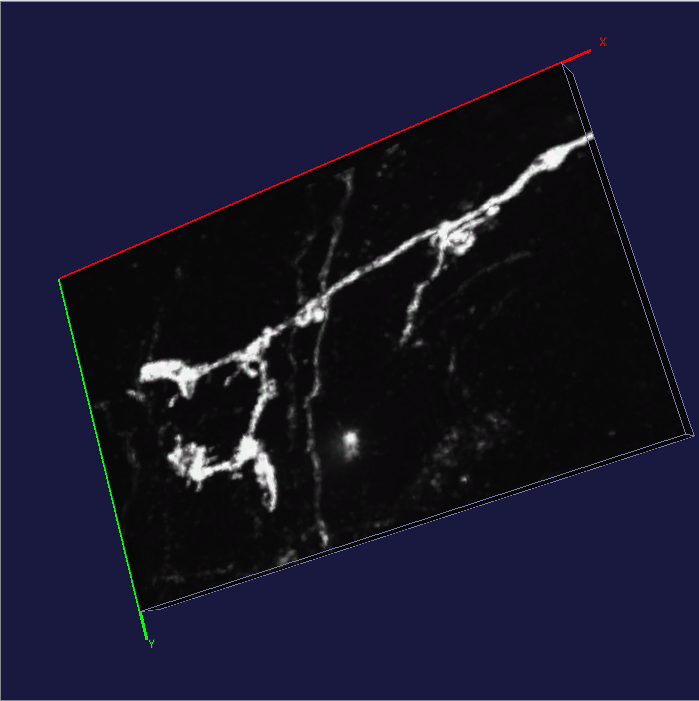
\includegraphics[width=.5\linewidth]{./images/TuFF/orig} \\
		\scriptsize (a) 3D neuron image
	\end{tabular}
	\\
	\begin{tabular}{cc}
		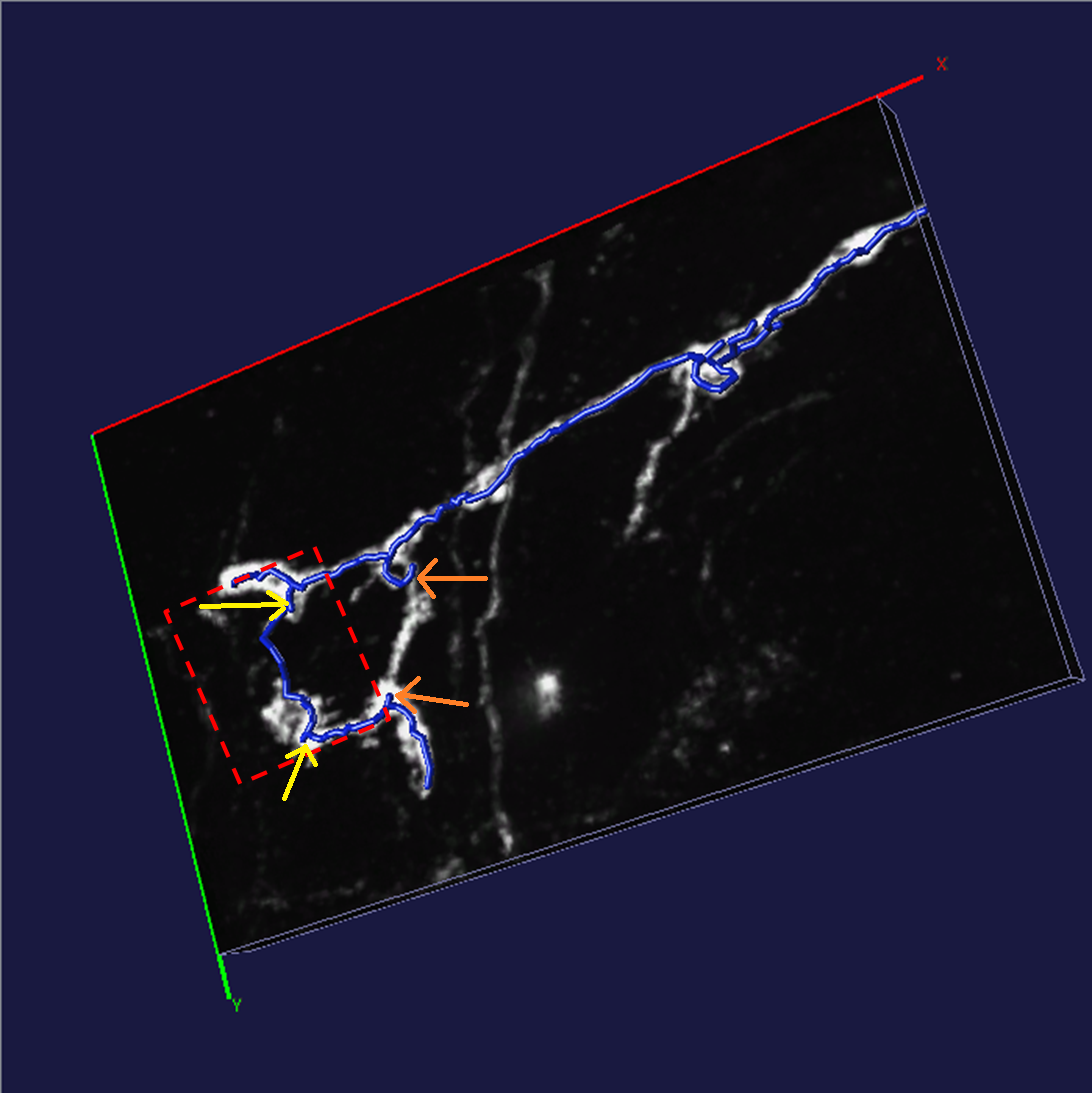
\includegraphics[width=.5\linewidth]{./images/TuFF/TypeB} &
		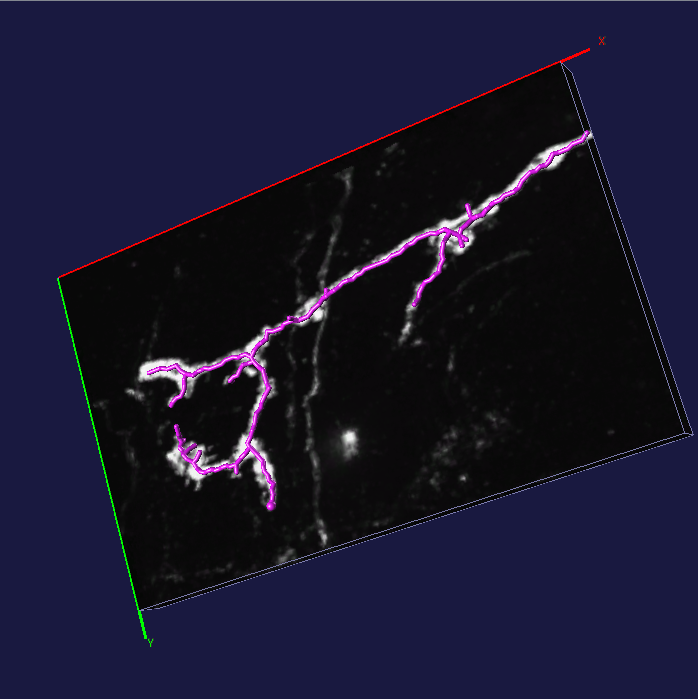
\includegraphics[width=.5\linewidth]{./images/TuFF/TypeBTuFF} \\
		\scriptsize(b) Tree2Tree & \scriptsize(c) TuFF
	\end{tabular}
\caption[TuFF vs Tree2Tree for type B connection (3D)]{An example in 3D where TuFF avoids type B connectivity error. (a) A 3D confocal microscopy image of a neuron is shown. (b) The tracing results of Tree2Tree is shown in blue. Tree2Tree causes type B error, shown by the yellow arrows. The actual connection should have been between the segments marked by orange arrows. (c) Tracing result due to TuFF is shown in magenta. This figure is best viewed in color.}
\label{fig:TypeB3D}
\end{figure}
To set up Tree2Tree for segmentation, we follow the author's methodology of performing an initial segmentation to obtain a set of binary components. The component analysis stage of Tree2Tree then decides on the connection between the segments by analyzing their relative orientation. To initialize the level set for TuFF, we have used Otsu's segmentation, same as Tree2Tree, and the level set propagates according to (\ref{eq:total_force_eqn}). Fig.~\ref{fig:Tuff_vs_T2T} demonstrates an example where Tree2Tree creates improper connection, due to its inability to handle type B discontinuity. The level set based methodology in TuFF performs proper segmentation (shown in Fig.~\ref{fig:Tuff_vs_T2T}(c),(d)). It is evident that the type B gap is closed by TuFF, where Tree2Tree fails to do so (see Fig.~\ref{fig:Tuff_vs_T2T}(c) vs (e)).


Two more examples are shown in Fig.~\ref{fig:twoD_comp_i} where Tree2Tree's tracing (shown in blue) creates incorrect branch connection as compared to TuFF (shown in magenta). The connection errors are highlighted by  the yellow arrows. Tree2Tree segmentation results suggest lack of robustness of the component linking scheme for complex structures embedded in a noisy environment. Furthermore the initial segmentation step in Tree2Tree often fails to detect low contrast objects, which cannot be recovered in future, since the multistage pipeline of Tree2Tree is unable to recover lost neurite portions. Fig.~\ref{fig:TypeB3D} demonstrates another example, for the 3D case, where TuFF performs robust segmentation of the neurites compared to Tree2Tree (Fig.~\ref{fig:TypeB3D}(c)), where connectivity error due to Type B discontinuity is observed (Fig.~\ref{fig:TypeB3D}(b)).   

The above examples suggest that TuFF handles bifurcations and component gaps successfully, since level sets are well equipped in handling topological changes. Also, the specially designed attraction force component of TuFF makes segmentation robust in cases where structure gaps result from very weak signal intensity (Fig.~\ref{fig:Tuff_vs_T2T}). 

\subsection{3D segmentation via TuFF: qualitative results}
\begin{figure}[h]
\centering
\renewcommand{\tabcolsep}{0.05cm}
	\begin{tabular}{@{}ccc @{}}
		\includegraphics[width=.33\linewidth]{./images/TuFF/qual3D/orig1_res} &
		\includegraphics[width=.33\linewidth]{./images/TuFF/qual3D/orig2_res} &		
		\includegraphics[width=.33\linewidth]{./images/TuFF/qual3D/orig4_res} \\		
		\includegraphics[width=.33\linewidth]{./images/TuFF/qual3D/orig1_swc} &
		\includegraphics[width=.33\linewidth]{./images/TuFF/qual3D/orig2_swc} &	
%		\includegraphics[width=.34\linewidth]{./images/TuFF/qual3D/orig3_res} &
%		\includegraphics[width=.34\linewidth]{./images/TuFF/qual3D/orig3_swc} \\
		\includegraphics[width=.33\linewidth]{./images/TuFF/qual3D/orig4_swc} 
	\end{tabular}
\caption[TuFF tracing results in 3D]{A few 3D neuron reconstruction examples using TuFF. The images are from the Condron dataset. The first row shows reconstructed neurites, overlaid on the original stack. The 3D reconstructions are shown in the second row. }
\label{fig:TuFF_recons}
\end{figure}
\noindent Fig.~\ref{fig:TuFF_recons} shows a few 3D neuron reconstructions (tracings) of Drosophila neurons using TuFF for segmentation. Digital reconstruction is obtained by computing the centerline of the segmented neuron, followed by spline fitting to each branch of the resulting skeleton graph. The neuron tracing results are shown in magenta, in the first row. The second row shows the neuronal structure, which is embedded in a \textit{.swc} file format. We have used the Vaa3D\cite{peng_v3d} toolkit for visualizing these digital reconstructions.

\subsection{Comparison of segmentation performance}
In this section we present a comparative segmentation performance analysis of the proposed method TuFF versus three popularly used neuron tracers. The ground truth data for segmentation is obtained by manually selecting points on the neuron structure and joining them manually in a manner that the morphological structure is preserved. The Vaa3d software \cite{peng_v3d} is used for creating the ground truth. To evaluate the performance of TuFF, we compare its performance to the following algorithms. 
\subsubsection{Graph Augmented Deformable (GD) model \cite{peng_GAD}} 
This semi automatic tool is extensively used for its relatively simple working methodology, which consists of a manual seed selection step followed by automated seed joining process by using graph theoretic techniques. Since the algorithm's efficacy is inversely proportional to the spatial distribution of selected seed points, we only select the neuron terminal points as the set of seeds. As the seed selection is performed manually, a practice which TuFF avoids, we believe that selecting the minimal set of seeds is essential to maintain fairness of comparison. Sample tracing results using this algorithm are shown in yellow.

\subsubsection{Neuronstudio \cite{rodriguez_voxelscoop}}
Neuronstudio is one of the state of the art publicly available automatic neuron segmentation software which is heavily used by biologists for tracing purpose. We have seen that segmentation accuracy of NeuronStudio is affected by the choice of the initial seed point. For each image in our dataset, we experiment with several initial seed locations and finally choose the one which yields the best visual segmentation result. Neuronstudio segmentation results are shown in orange color.

\subsubsection{Tree2Tree \cite{basu_T2T_journal}}
As discussed earlier, Tree2Tree belongs to the category of seed independent neron segmentation methods. Setting up Tree2Tree requires an initial segmentation stage, followed by graph-theoretic component linking procedure. The segmentation results of Tree2Tree are shown in blue color.

For each of the above mentioned algorithms and TuFF, we first obtain the segmentation followed by neuron centerline detection. A cubic spline is fitted to each branch of the detected centerline. This spline fitted centerline of the neurons represent the tracing results.
\begin{figure}[t]
\centering
\subfigure{
	\renewcommand{\tabcolsep}{0.05cm}
	\begin{tabular}{@{}cccccc @{}}
		\includegraphics[width=.16\textwidth]{./images/3D_results/in44_body_orig} &
		\includegraphics[width=.16\textwidth]{./images/3D_results/in44_body_ground} &
		\includegraphics[width=.16\textwidth]{./images/3D_results/in44_body_peng} & 
		\includegraphics[width=.16\textwidth]{./images/3D_results/in44_body_NS} &
		\includegraphics[width=.16\textwidth]{./images/3D_results/in44_body_T2T} &
		\includegraphics[width=.16\textwidth]{./images/3D_results/in44_body_MFVF}
		\\
		\includegraphics[width=.16\textwidth]{./images/3D_results/M4_1_orig} &
		\includegraphics[width=.16\textwidth]{./images/3D_results/M4_1_ground} &
		\includegraphics[width=.16\textwidth]{./images/3D_results/M4_1_peng} & 
		\includegraphics[width=.16\textwidth]{./images/3D_results/M4_1_NS} &
		\includegraphics[width=.16\textwidth]{./images/3D_results/M4_1_T2T} &
		\includegraphics[width=.16\textwidth]{./images/3D_results/M4_1_MFVF} 
		\\
		\includegraphics[width=.16\textwidth]{./images/3D_results/M4_5_orig} &
		\includegraphics[width=.16\textwidth]{./images/3D_results/M4_5_ground} &
		\includegraphics[width=.16\textwidth]{./images/3D_results/M4_5_peng} & 
		\includegraphics[width=.16\textwidth]{./images/3D_results/M4_5_NS} &
		\includegraphics[width=.16\textwidth]{./images/3D_results/M4_5_T2T} &
		\includegraphics[width=.16\textwidth]{./images/3D_results/M4_5_MFVF} 
		\\
		\includegraphics[width=.16\textwidth]{./images/3D_results/M4_9_orig} &
		\includegraphics[width=.16\textwidth]{./images/3D_results/M4_9_ground} &
		\includegraphics[width=.16\textwidth]{./images/3D_results/M4_9_peng} & 
		\includegraphics[width=.16\textwidth]{./images/3D_results/M4_9_NS} &
		\includegraphics[width=.16\textwidth]{./images/3D_results/M4_9_T2T} &
		\includegraphics[width=.16\textwidth]{./images/3D_results/M4_9_MFVF}
		\\
		\includegraphics[width=.16\textwidth]{./images/3D_results/M4_6_orig} &
		\includegraphics[width=.16\textwidth]{./images/3D_results/M4_6_ground} &
		\includegraphics[width=.16\textwidth]{./images/3D_results/M4_6_peng} & 
		\includegraphics[width=.16\textwidth]{./images/3D_results/M4_6_NS} &
		\includegraphics[width=.16\textwidth]{./images/3D_results/M4_6_T2T} &
		\includegraphics[width=.16\textwidth]{./images/3D_results/M4_6_MFVF}  
		\\
		\scriptsize(a) 3D stack & 
		\scriptsize(b) Ground truth &
		\scriptsize(c) GD model \cite{peng_GAD} & 
		\scriptsize(d) NeuronStudio \cite{rodriguez_voxelscoop} & 
		\scriptsize(e) Tree2Tree \cite{basu_T2T_journal} & 
		\scriptsize(f) TuFF
	\end{tabular}
} 
\caption[TuFF tracing results -- 1]{Tracing results on 3D images of the UVA-Condron dataset. First column shows the original images, followed by the tracing outputs of the different algorithms. Tracing results of TuFF are shown in the last column in magenta.}
\label{fig:threeD_comp_i}
\end{figure}

\subsection{Qualitative performance analysis}

\subsubsection{Results on Condron data set}
Fig.~\ref{fig:threeD_comp_i} shows the performance of the above mentioned neuron tracers on five representative neurons chosen from the Condron dataset. The 3-D stacks are shown in the first column, followed by manual ground truth segmentation in the second column (shown in green). Tracing results using GD model \cite{peng_GAD} is plotted in yellow in the third column. The fourth and fifth columns show segmentation output using the automated techniques Neuronstudio and Tree2Tree (plotted in orange and blue color) respectively. Finally, the last column shows the neuron tracing due to TuFF (plotted in magenta).

It may be observed that these images are in general noisy, which makes the segmentation task difficult. Moreover, high structural complexity of the neurons require sophisticated mechanism to preserve the structural morphology. The severity of contrast variation and low SNR pose difficulty for the GD model. Even with manually selected terminal nodes, it is seen that the semi-manual tracer performs incorrect segmentation (Fig.~\ref{fig:threeD_comp_i}, second column, rows 2-5). This is primarily due to the inability of the local search based technique fails to identify the actual filamentous path in presence of clutter. Furthermore, human assisted neurite termination detection proved to be a difficult and time consuming problem in these images owing to the high structural complexity. 

Neuronstudio performs particularly poorly in these examples. The major reason can be attributed to the lack of continuity in the neurite structure and high signal variation, which forces the algorithm to converge prematurely. Also, the cluttered environment is detrimental to the performance of the local voxel scooping process of Neuronstudio. This results in under segmentation and sometimes, incorrect segmentation due to leakage of the region growing technique.

Tree2Tree outperforms Neuronstudio, especially when the component linking algorithm is able to determine proper connectivity. We observe that Tree2Tree performs well if the initial segmentation step is reliable. However, under segmentation is an inherent problem in Tree2Tree due its inability to incorporate additional neuronal structures in its solution after initial thresholding.

On the other hand, TuFF performs segmentation efficiently, even in cluttered environment. A close inspection would reveal that important morphological entities like bifurcation points and branch locations are preserved (see Fig.~\ref{fig:threeD_comp_i} rows 2,3 and 4), while the iterative directional region growing scheme prevents under segmentation of neurons. 

\subsubsection{Segmentation results on OP dataset} These image stacks exhibit relatively higher signal intensity than the Condron data set. However, neuron tracing is still a challenging task owing to their complicated structure and sudden intensity variations in the neurites, creating a fragmented, discontinuous appearance. This often results in type B discontinuity which demands sophisticated analysis. Fig.~\ref{fig:threeD_comp_ii} compares the segmentation results for  above mentioned algorithms.

Reduction in background clutter and increased signal intensity assists the semi automatic GD-model tracer. Since the images exhibit significant improvement in contrast, manual detection of seeds is less stressful. Still, the complicated structure of a few images (Fig.~\ref{fig:threeD_comp_ii}, row 1 for example) makes manual seed selection demanding. Performance of Neuronstudio also shows slight improvement in this dataset. However, despite brighter foreground and less noise, this local tracing scheme shows tendency to stop at intensity gaps, which needs to be modified manually at a later stage.
\begin{figure}[t]
\centering
\subfigure{
	\renewcommand{\tabcolsep}{0.05cm}
	\begin{tabular}{@{}cccccc @{}}
		\includegraphics[width=.16\textwidth]{./images/3D_results_2/OP1_orig} &
		\includegraphics[width=.16\textwidth]{./images/3D_results_2/OP1_ground} &
		\includegraphics[width=.16\textwidth]{./images/3D_results_2/OP1_peng} & 
		\includegraphics[width=.16\textwidth]{./images/3D_results_2/OP1_NS} &
		\includegraphics[width=.16\textwidth]{./images/3D_results_2/OP1_T2T} &
		\includegraphics[width=.16\textwidth]{./images/3D_results_2/OP1_MFVF}
		\\
		\includegraphics[width=.16\textwidth]{./images/3D_results_2/M4_7_orig} &
		\includegraphics[width=.16\textwidth]{./images/3D_results_2/M4_7_ground} &
		\includegraphics[width=.16\textwidth]{./images/3D_results_2/M4_7_peng} & 
		\includegraphics[width=.16\textwidth]{./images/3D_results_2/M4_7_NS} &
		\includegraphics[width=.16\textwidth]{./images/3D_results_2/M4_7_T2T_changed} &
		\includegraphics[width=.16\textwidth]{./images/3D_results_2/M4_7_MFVF} 
		\\
		\includegraphics[width=.16\textwidth]{./images/3D_results_2/OP7_orig} &
		\includegraphics[width=.16\textwidth]{./images/3D_results_2/OP7_ground} &
		\includegraphics[width=.16\textwidth]{./images/3D_results_2/OP7_peng} & 
		\includegraphics[width=.16\textwidth]{./images/3D_results_2/OP7_NS} &
		\includegraphics[width=.16\textwidth]{./images/3D_results_2/OP7_T2T} &
		\includegraphics[width=.16\textwidth]{./images/3D_results_2/OP7_MFVF}
		\\
		\includegraphics[width=.16\textwidth]{./images/3D_results_2/OP9_orig} &
		\includegraphics[width=.16\textwidth]{./images/3D_results_2/OP9_ground} &
		\includegraphics[width=.16\textwidth]{./images/3D_results_2/OP9_peng} & 
		\includegraphics[width=.16\textwidth]{./images/3D_results_2/OP9_NS} &
		\includegraphics[width=.16\textwidth]{./images/3D_results_2/OP9_T2T} &
		\includegraphics[width=.16\textwidth]{./images/3D_results_2/OP9_MFVF}
		\\
		\scriptsize(a) 3D stack & 
		\scriptsize(b) Ground truth &
		\scriptsize(c) GD model \cite{peng_GAD} & 
		\scriptsize(d) NeuronStudio \cite{rodriguez_voxelscoop} & 
		\scriptsize(e) Tree2Tree \cite{basu_T2T_journal} & 
		\scriptsize(f) TuFF
	\end{tabular}
} 
\caption[TuFF tracing results -- 2]{Results on the images of the OP dataset. First column shows the original images, followed by the tracing outputs of the different algorithms. Tracing results of TuFF are shown in the last column in magenta. }
\label{fig:threeD_comp_ii}
\end{figure}
On the other hand, it is observed that Tree2Tree's performance degrades significantly for this dataset. This is primarily due to a large number of improper branch connections. This connectivity error occurs mostly due to Tree2Tree's inability to handle type B discontinuities (Fig.~\ref{fig:threeD_comp_ii}, rows 1-3). In fact, even in relatively high SNR images Tree2Tree under performs significantly by extracting an improper structural morphology of the neurons. TuFF, however demonstrates good performance on these images by virtue of its ability to handle structure gaps automatically. The segmentation results are shown in the last column of Fig.~\ref{fig:threeD_comp_ii}. A qualitative assessment of the algorithm's performance is presented in the following sections.


\subsection{Quantitative Performance Analysis}
\begin{figure}[b]
\renewcommand{\tabcolsep}{0.05cm}
\begin{tabular}{cc}
	\includegraphics[width=.48\linewidth]{./images/TuFF/FP}
	&\includegraphics[width=.48\linewidth]{./images/TuFF/FN}
	\\
	\scriptsize (a) False positives & \scriptsize (b) False negatives
	\\
	\includegraphics[width=.48\linewidth]{./images/TuFF/wrong}
	&\includegraphics[width=.48\linewidth]{./images/TuFF/MAE} \\
	\scriptsize (c) Incorrect connection & \scriptsize (d) MAE
\end{tabular}
\caption[Quantitative performance comparison]{(a)-(c): Quantitative performance of the four neuron tracers TuFF (pink), Neuron Studio (orange), GD model \cite{peng_GAD} (yellow) and Tree2Tree (blue) in terms of number of over-estimated branches, number of under-estimated branches and total number of wrong connections respectively. (d) quantifies the tracing accuracy in terms of mean absolute error (\ref{eq:MEA}).}
\label{fig:graph_plots}
\vspace{-0.2in}
\end{figure}
To quantify the segmentation performance, we identify four measures which reflects the efficiency of a particular neuron tracer. These are as follows: number of over-estimated branches (Fig.~\ref{fig:graph_plots}(a)), number of unidentified/missed branches (Fig.~\ref{fig:graph_plots}(b)), total number of incorrect branch connections (see Fig.~\ref{fig:graph_plots}(c)) and finally the mean absolute error in the traced centerline with respect to the ground truth.

The number of over determined/missed branches reflect the adequacy of an algorithm in respecting the morphology of the imaged neuronal structure. This quantification of the segmentation quality is performed by a human expert. However, since even the ground truth data is susceptible to subtle errors in computing the 3D skeleton, we have disregarded small branches (less than 5 units in length) from the analysis. The graphs in Fig.~\ref{fig:graph_plots}(a) and (b) suggests that over the whole data set, TuFF outperforms the competing algorithms in a majority of cases. It is observed in a few cases that Neuronstudio in particular misses a large number of branches, due to its inability to deal with fragmented structure.



The number of incorrect branch connections (Fig.~\ref{fig:graph_plots}(c)) indicate an algorithm's ability to tackle discontinuities. Indeed, improper connections often result when signal heterogeneity is significant. Apart from a few occasions, TuFF demonstrates its superiority in handling discontinuities better than other automated methods.    

To perform quantitative analysis of the traced neuron centerline, we compute the mean absolute error (MAE) of the obtained trace against the manually acquired ground truth. If $\mathcal{P}=\{p_1,\ldots,p_n\}$ and $\mathcal{Q}=\{q_1,\ldots,q_m\}$ denote the set of traced coordinates for a neuron, the mean absolute error (in pixels) between the traces is given by
\bea
\text{MAE}=\frac{1}{n}\sum_{i=1}^{n} \min_j|p_i-q_j| +
             \frac{1}{m}\sum_{i=1}^{m} \min_k|q_i-p_k| 
\label{eq:MEA}
\eea
$\forall j\in\{1,..,m\}$, $\forall k\in\{1,..,n\}$. Mean absolute errors for the 3-D images are plotted for each algorithm in Fig.~\ref{fig:graph_plots}(d). It is observed that TuFF outperforms the automated tracers Tree2Tree and Neuronstudio in almost all of the cases, except for the $8^{\text{th}}$ and $16^{\text{th}}$ stack, where Tree2Tree and Neuronstudio perform marginally better. Also, TuFF successfully competes with the semi-automatic GD-model, even outperforming it in some images in the Condron dataset. 
\begin{table}[b]
    	\caption[Quantitative analysis of TuFF]{Comparison of MAE}
	\centering
    \begin{tabular}{lcccc}
%    \hline
    ~               & \textbf{TuFF} & \textbf{Neuron Studio} &\textbf{ GD model} & \textbf{Tree2Tree} \\ 
%    \hline
    Avg. MAE    & 8.81 & 79.98         & 15.41     & 17.62      \\
    Median MAE  & 7.95 & 34.06          & 8.54     & 13.98      \\
    Std. Dev        & 3.4 & 50.6          & 14.03     & 15.08      \\ 
%    \hline
    \end{tabular}
\label{table:quant_compare}
\end{table}

The mean, median and standard deviation MAE of the four algorithms are reported in Table~\ref{table:quant_compare}. This suggests that on a whole TuFF outperforms its competitors with a mean and median MAE of 8.81 (pixels) and 7.95 (pixels) respectively. TuFF also exhibits 75\% improvement of mean error over the second best performer, which is the semi-automatic tracer of Peng \textit{et al}. If we compare its efficacy against the fully automated techniques, we obtain an improvement of over 98\% over Tree2Tree, while Neuron Studio is outperformed with an improvement of greater than 400\%. Also, the error standard deviation of TuFF is only 3.4 as compared to 50.6, 14.03 and 15.08 for Neuronstudio, GD-model and Tree2Tree. The visual segmentation results and the quantitative results presented here suggests the efficiency of TuFF in segmenting structurally complex neurons from cluttered confocal microscope images.

\section{Further improvements}

Until now, we have described the application of TuFF for the purpose of segmenting neurons from 2D and 3D imagery. However, the basic formulation of TuFF is applicable to other segmentation problems, which involve tubular objects. As a result, the mathematical formulation of TuFF involves a technique for identifying the tubular structures from the noisy images. The hessian based methodology of Frangi \cite{frangi_vesselness} is used here, as well as in Tree2Tree-2, to get a vesselness function and the vessel orientations. However, this popular tool has a severe drawback; it is unable to detect key locations such as filament bifurcations and end points. Furthermore, the obtained vesselness response diminishes directly with the vessel signal intensity. Therefore, in many cases, the Frangi filter produces nonlinear vesselness maps with significant false negatives at vessel junctions, terminals or at locations with relatively lower foreground intensity. This creates major hurdles in Tree2Tree/Tree2Tree-2 \cite{basu_T2T_journal,mukherjee_T2T_2}, and while the local attraction force in TuFF tries to mitigate this artifact, we hypothesize that a robust vessel identification scheme would result in refined segmentation. The proposed method uses specialized steerable filters for ridge detection that incorporates a local processing scheme to enhance vessel detection. Finally, we show that in the  variational paradigm, it is also possible to incorporate edge based energy term in the TuFF equation, which can assist segmentation in some applications.
The extensions of  TuFF and a few non biological applications are discussed in    Appendix \ref{AppendixLDE}. 


\section{Discussion}

In this paper we have presented an automated neuron segmentation algorithm which can segment neurons from both 2-D and 3-D images. The proposed framework is suitable for tracing highly fragmented neurite images, and is capable of processing the structure discontinuities automatically, while respecting the overall neuron morphology. Connectivity analysis is performed in a level set framework which presents a nice and simple alternative to graph based techniques which may introduce undesired branches in segmentation. The efficiency of TuFF is further demonstrated by its superior overall quantitative performance where it outperforms peer algorithms, including a semi manual tracer. The salient highlights of this proposed method is discussed below.

First, we avoid human intervention in terms of seed point selection. Automated initialization of the level set is performed by Otsu's global thresholding \cite{otsu} followed by noise removal using morphological area open operators \cite{acton_fast}. The level set function is computed from this initialized segments using binary distance transform.

Second, TuFF presents a natural framework to process both type A and type B discontinuities (Fig.~\ref{fig:typeAB_demo}). This is a major improvement over  Tree2Tree \cite{basu_T2T_journal}, where the inability to handle type B discontinuity introduces several false connections in the solution. 

Finally, TuFF is capable of joining broken neurite fragments even in complete absence of signal. The proposed attraction force field is independent of the local signal intensity and depends only on the morphology and relative positioning of the connected components. This feature improves on the widely used local intensity seeking neuron tracers \cite{rodriguez_voxelscoop}, which are susceptible to illumination variation in the images of neural structure. The TuFF guided evolution energy is combined with the attraction force component in a mathematically elegant, integrated fashion as opposed to a multistage sequential processing pipeline.











